
\section{Reproducibility and Deployment Details}
\label{app:reproducibility}

The main paper makes a simple claim: safe Kubernetes autoscaling is not
only a control problem, but a world-modeling problem.  A controller that
reacts only after pressure appears is always one step behind; a
controller that over-provisions everywhere buys safety too expensively.
NetDream takes the third path: it learns a compact graph world model,
uses it to imagine the near future, and then acts only on futures that
look safe.

This first appendix section opens the box.  It shows that the main
results do not depend on a large hidden system or fragile engineering
tricks.  NetDream is a small residual GAT, trained offline from logged
transitions, and queried online by a short-horizon planner.  We first
give the exact hyperparameters, then show the training and compute
profile, and finally describe the runtime controller used in the AWS EKS
deployment.

\subsection{Model, Training, and Planning Configuration}
\label{app:hyperparams}

The key design choice is to keep the world model small enough to be
operational.  The model must be expressive enough to predict how load and
latency propagate through a microservice graph, but cheap enough to be
queried many times inside a planning loop.  NetDream therefore uses a
3-layer graph attention network with residual dynamics and three heads:
one for next-state prediction, one for reward, and one for constraint
risk.  Table~\ref{tab:hyperparams} gives the exact configuration used
throughout the Kubernetes experiments unless otherwise stated.

\begin{table}[H]
\centering
\small
\caption{NetDream hyperparameter configuration.}
\label{tab:hyperparams}
\begin{tabular}{@{}ll@{}}
\toprule
\textbf{Parameter} & \textbf{Value} \\
\midrule
\multicolumn{2}{@{}l}{\textit{GNN Dynamics Model}} \\
GNN type & GAT (4 heads) \\
Hidden dimension & 128 \\
Number of GNN layers & 3 \\
Residual connections & Yes \\
Dropout & 0.0 \\
Total parameters & 86,536 (K8s) / 86,793 (Grid) \\
\midrule
\multicolumn{2}{@{}l}{\textit{Training}} \\
Optimizer & Adam \\
Learning rate & $3 \times 10^{-4}$ \\
Weight decay & $1 \times 10^{-5}$ \\
Batch size & 128 \\
Max epochs & 100 \\
Early stopping patience & 15 \\
Gradient clip norm & 1.0 \\
Loss weights ($\alpha$, $\beta$) & 0.1, 0.1 \\
\midrule
\multicolumn{2}{@{}l}{\textit{Planning}} \\
Planner type & Batched random shooting \\
Number of candidates ($K$) & 64 \\
Planning horizon ($H$) & 5 \\
No-op bias & 70\% \\
Safety threshold ($\tau$) & 0.5 \\
\midrule
\multicolumn{2}{@{}l}{\textit{PPO Baseline}} \\
Algorithm & PPO (Stable-Baselines3) \\
Network & MLP [64, 64] \\
Training steps & 500,000 \\
Learning rate & $3 \times 10^{-4}$ \\
\midrule
\multicolumn{2}{@{}l}{\textit{Data Collection}} \\
K8s transitions & 48,000 (200 ep $\times$ 240 steps) \\
Grid2Op transitions & 12,040 (200 ep) \\
WaterNet-10 transitions & 19,200 (200 ep $\times$ 96 steps) \\
EpiNet-20 transitions & 12,000 (200 ep $\times$ 60 steps) \\
Train/val split & 80\% / 20\% \\
Random seeds & $\{42, 123, 456, 789, 1024\}$ \\
\bottomrule
\end{tabular}
\end{table}

Table~\ref{tab:hyperparams} also highlights the two constraints that
shape the method: the model must be small enough for online planning, and
the planner must be conservative enough to avoid unsafe futures.  The
next two paragraphs show that these constraints are satisfied in
practice.

\paragraph{Training behavior.}
After fixing the model size, the next question is whether such a small
world model can actually learn useful Kubernetes dynamics.  The answer is
yes: validation loss stabilizes by roughly epoch 30 and continues to
improve slightly through epoch 100, without visible overfitting.  This
supports a key design choice of the paper: NetDream does not require a
massive model or unsafe online reinforcement learning to become useful;
a compact offline-trained graph dynamics model is sufficient for
short-horizon imagination.

\begin{table}[H]
\centering
\small
\caption{Training convergence: validation loss by epoch (K8s GAT model).
Early stopping triggered at epoch 100 (patience 15).}
\label{tab:training}
\begin{tabular}{@{}lcccc@{}}
\toprule
Epoch & Train Loss & Val Loss & Best Val & Learning Rate \\
\midrule
1 & 0.01052 & 0.00819 & 0.00819 & $3\!\times\!10^{-4}$ \\
10 & 0.00485 & 0.00495 & 0.00495 & $3\!\times\!10^{-4}$ \\
30 & 0.00416 & 0.00424 & 0.00424 & $3\!\times\!10^{-4}$ \\
50 & 0.00381 & 0.00421 & 0.00412 & $3\!\times\!10^{-4}$ \\
80 & 0.00328 & 0.00408 & 0.00405 & $3\!\times\!10^{-4}$ \\
100 & 0.00307 & 0.00402 & 0.00400 & $3\!\times\!10^{-4}$ \\
\bottomrule
\end{tabular}
\end{table}

Thus, the world model reaches a useful validation regime quickly.  The
next question is whether this learned model can be queried fast enough
inside a repeated planning loop.

\paragraph{Computation.}
This small-model design also matters at deployment time.  The planner
queries the world model repeatedly, so inference latency must be far
below the control interval.  In practice, the full experimental pipeline
is lightweight: the Kubernetes model trains in minutes, and each online
planning step takes less than 10 ms, well below the interval used in our
deployment.

\begin{table}[H]
\centering
\small
\caption{Wall-clock time for each component on a single NVIDIA GPU.}
\label{tab:compute}
\begin{tabular}{@{}lcc@{}}
\toprule
Component & K8s Mesh & Power Grid \\
\midrule
Data collection (200 episodes) & 2 min & 8 min \\
Model training (100 epochs) & 5 min & 3 min \\
Planning evaluation (3 seeds $\times$ 4 workloads) & 15 min & 5 min \\
GNN ablation (4 variants) & 20 min & -- \\
\midrule
Total & $\sim$42 min & $\sim$16 min \\
\bottomrule
\end{tabular}
\end{table}

These runtime numbers justify the use of model-predictive planning rather
than a single direct policy lookup: NetDream can afford to evaluate many
imagined futures before acting.

\subsection{Algorithms}
\label{app:pseudocode}

The method has two phases, mirroring the story in the main paper.  In
the offline phase, NetDream learns the local physics of the service graph:
how the current state and a candidate scaling action change future
metrics, rewards, and risk.  In the online phase, NetDream turns this
model into a decision mechanism: it samples possible scaling futures,
rolls them forward in imagination, rejects unsafe ones, and executes only
the first action of the best remaining plan.  Algorithms~\ref{alg:training}
and~\ref{alg:planning} give the exact procedures.

\begin{algorithm}[H]
\caption{NetDream Dynamics Model Training}
\label{alg:training}
\begin{algorithmic}[1]
\REQUIRE Transition dataset $\mathcal{D} = \{(G, z_t, a_t, z_{t+1}, r_t, c_t)\}$,
         GNN type $\in \{\texttt{gat}, \texttt{gcn}, \texttt{sage}\}$,
         hidden dimension $d = 128$, epochs $E = 100$
\ENSURE Trained dynamics model $f_\theta$
\STATE Initialize $f_\theta$ with Xavier weights
\STATE Split $\mathcal{D}$ into train/val at 80/20
\FOR{epoch $= 1$ to $E$}
  \FOR{each mini-batch $\mathcal{B} \subset \mathcal{D}_{\text{train}}$}
    \FOR{$(G, z_t, a_t, z_{t+1}, r_t, c_t) \in \mathcal{B}$}
      \STATE $h \leftarrow \text{NodeEncoder}([z_t \,\|\, \text{OneHot}(a_t)])$
      \FOR{$k = 1$ to $K_{\text{layers}}$}
        \STATE $h \leftarrow \text{GNNLayer}_k(h, \mathcal{E}) + h$
        \STATE $h \leftarrow \text{LayerNorm}(h)$
      \ENDFOR
      \STATE $\hat{\Delta z} \leftarrow \text{DynamicsHead}(h)$
      \STATE $\hat{r} \leftarrow \text{RewardHead}(h)$
      \STATE $\hat{c} \leftarrow \sigma(\text{ConstraintHead}(h))$
      \STATE $\mathcal{L} \leftarrow \|\hat{\Delta z} - (z_{t+1} - z_t)\|^2
             + \alpha\|\hat{r} - r_t\|^2
             + \beta\, \text{BCE}(\hat{c}, c_t)$
    \ENDFOR
    \STATE Update $\theta \leftarrow \theta - \eta \nabla_\theta \mathcal{L}$
      \COMMENT{Adam, $\eta = 3 \times 10^{-4}$, clip norm 1.0}
  \ENDFOR
  \IF{val loss has not improved for 15 epochs}
    \STATE \textbf{break}
  \ENDIF
\ENDFOR
\RETURN $f_\theta$
\end{algorithmic}
\end{algorithm}

\begin{algorithm}[H]
\caption{NetDream-Safe: Imagination-Based MPC with Safety Filter}
\label{alg:planning}
\begin{algorithmic}[1]
\REQUIRE Trained model $f_\theta$, current state $z_t$, graph $G$,
         candidates $K = 64$, horizon $H = 5$, safety threshold $\tau = 0.5$,
         no-op bias $\rho = 0.7$
\ENSURE Action $a_t^*$ to execute
\FOR{$k = 1$ to $K$}
  \FOR{$h = 1$ to $H$}
    \STATE $a^{(k)}_h \sim \text{Uniform}(\{-1,0,+1\}^n)$
      with probability $\rho$ replaced by no-op $\mathbf{0}$
  \ENDFOR
\ENDFOR
\FOR{$k = 1$ to $K$}
  \STATE $z^{(k)}_0 \leftarrow z_t$,\quad safe$^{(k)} \leftarrow$ true,
         \quad $R^{(k)} \leftarrow 0$
  \FOR{$h = 1$ to $H$}
    \STATE $(\hat{\Delta z}, \hat{r}, \hat{c}) \leftarrow f_\theta(G, z^{(k)}_{h-1}, a^{(k)}_h)$
    \STATE $z^{(k)}_h \leftarrow z^{(k)}_{h-1} + \hat{\Delta z}$
    \STATE $R^{(k)} \leftarrow R^{(k)} + \hat{r}$
    \IF{$\hat{c} > \tau$}
      \STATE safe$^{(k)} \leftarrow$ false;\quad \textbf{break}
    \ENDIF
  \ENDFOR
\ENDFOR
\STATE $\mathcal{S} \leftarrow \{k : \text{safe}^{(k)} = \text{true}\}$
\IF{$\mathcal{S} \neq \emptyset$}
  \STATE $k^* \leftarrow \arg\max_{k \in \mathcal{S}} R^{(k)}$
  \RETURN $a^{(k^*)}_1$
\ELSE
  \RETURN $\mathbf{0}$ \COMMENT{safe default: hold current replicas}
\ENDIF
\end{algorithmic}
\end{algorithm}

The two algorithms describe the computation; the next subsection
describes how that computation is embedded into a live Kubernetes
controller.

\subsection{Deployment Architecture on AWS EKS}
\label{app:deployment}

The algorithms above are not only simulator procedures.  They are wrapped
into a controller that runs against a real Kubernetes control plane.  The
runtime system has four components, each corresponding to one step in the
closed-loop control story: observe the cluster, build the graph state,
plan in the world model, and apply the selected scaling action.

\paragraph{State estimator.}
A Python service scrapes CPU utilization, replica counts, P95 latency,
QPS, error rates, and memory usage at 5-second intervals.  Raw metrics
are normalized using training-set statistics and formatted as a PyG
\texttt{Data} object with the Online Boutique topology.

\paragraph{NetDream inference service.}
The inference service receives the graph state, runs
Algorithm~\ref{alg:planning} on GPU, and emits per-service scaling
decisions $\{s_i:\delta_i\}_{i=0}^{10}$.

\paragraph{Kubernetes controller.}
A custom controller applies scaling decisions via the \texttt{/scale}
subresource on each \texttt{Deployment}.  Scale-down operations are
rate-limited to one replica per service per decision interval to prevent
oscillation; scale-up operations are applied immediately.

\paragraph{Monitoring and decision loop.}
Prometheus collects per-pod metrics, and Grafana visualizes SLO
compliance, replica counts, and fallback rate.  At each 15-second
interval, the system collects metrics, builds the graph state, runs
NetDream, and applies scaling decisions.  Total loop latency is below
200 ms, dominated by Prometheus scrape delay.

\paragraph{EKS configuration.}
Experiments run on a 3-node EKS cluster in \texttt{us-east-1}.  Online
Boutique pods are scheduled with resource requests but without hard
limits, allowing natural CPU throttling.  Locust runs in a dedicated
namespace to avoid interfering with service metrics.

\subsection{Reproducibility and Responsible Use}
\label{app:release-impact}

Taken together, the preceding details are meant to make NetDream
reproducible as a system, not only as a model.  All code, trained models,
collected data, cluster manifests, and evaluation scripts are included in
the supplementary material.  The Kubernetes simulator is implemented in
Python/NumPy with PyTorch and PyTorch Geometric.  EKS experiments use
seeds $\{42,123,456\}$; simulator ablations and prediction tables use
seeds $\{42,123,456,789,1024\}$.

The safety framing also deserves a careful interpretation.  NetDream
should be used as a complement to existing production safety mechanisms,
not as a replacement.  The safety filter can reject predicted unsafe
futures, but it remains limited by model accuracy.  In deployment, it
should be paired with standard safeguards such as circuit breakers,
rollback policies, and human oversight.

\section{Kubernetes Testbed and Full Empirical Results}
\label{app:k8s-full}

The main paper evaluates NetDream on Kubernetes because Kubernetes
autoscaling is exactly the setting where local actions have graph-level
consequences.  Scaling the frontend may relieve one bottleneck while
shifting pressure to checkout, cart, or recommendation services.  This
section therefore moves from implementation to evidence: it first
describes the simulated and real Kubernetes environments, then specifies
the service graph and workload regimes, and finally reports the full
per-workload and per-seed results behind the aggregate Pareto frontier.

\subsection{Kubernetes Simulator and Real Cluster}
\label{app:k8s-sim}

We use the simulator for controlled training and diagnostics, and the EKS
cluster for the final closed-loop test.  The simulator is designed to
capture the phenomena that make autoscaling difficult: traffic fans out
through the graph, overloaded services create cascade penalties, new pods
are not ready immediately, and CPU responds to load per replica.  We
simulate Google Online Boutique with 11 services connected by 14 directed
API-call edges.  The GNN uses the bidirectional version of this graph.
The simulator models four effects: traffic propagation from the frontend
to downstream services, cascade penalties when callers approach the SLO
boundary, a 3-step pod startup delay for new replicas, and a CPU model of
\[
\text{CPU\%}=5+(\text{QPS}/\text{replicas})\times 0.7.
\]
The SLO violation indicator is triggered when p95 latency exceeds 500 ms
or error rate exceeds 5\%.

For real-cluster validation, Online Boutique is deployed on both a local
MicroK8s cluster and a production-grade AWS EKS cluster.  The local
cluster supports development and sanity checks; the EKS cluster is used
for final closed-loop evaluation.  Metrics are collected through
Prometheus, workloads are generated by Locust, and Cluster Autoscaler is
disabled so that pod-level replica decisions come only from the evaluated
autoscaler.

\begin{table}[H]
\centering
\small
\caption{EKS cluster statistics across all 85 evaluation episodes
(7 agents $\times$ 4 workloads $\times$ 3 seeds, 60 steps/episode).
All numbers are derived from raw \texttt{eks\_*.json} log files
recorded during the experiments.}
\label{tab:eks-stats}
\begin{tabular}{@{}ll@{}}
\toprule
\textbf{Parameter} & \textbf{Value} \\
\midrule
\multicolumn{2}{@{}l}{\textit{Cluster hardware}} \\
Node type & AWS t3.medium $\times$ 3 (2 vCPU, 4 GB RAM / node) \\
Total capacity & 6 vCPU, 12 GB RAM \\
Region & \texttt{us-east-1} \\
\midrule
\multicolumn{2}{@{}l}{\textit{Experiment scope}} \\
Total EKS episodes & 85 \\
Steps per episode & 60 (5-minute window at 5 s/step) \\
Total decision steps & 5{,}100 \\
Prometheus scrape points & 56{,}100 (85 ep $\times$ 60 steps $\times$ 11 services) \\
Total experiment wall time & 3.4 hours \\
\midrule
\multicolumn{2}{@{}l}{\textit{Pod scheduling activity}} \\
Replica range (per service) & 1--10 \\
Total cluster pods (per step) & 11--110 (mean 48.5) \\
Pod creation events & 6{,}529 \\
Pod deletion events & 6{,}384 \\
\midrule
\multicolumn{2}{@{}l}{\textit{Observed workload metrics}} \\
Frontend QPS & 0--96 req/s (mean 35) \\
Frontend latency & 180--2{,}000 ms (mean 552 ms) \\
Frontend error rate & 0.00\%--4.02\% \\
\bottomrule
\end{tabular}
\end{table}

These statistics confirm that the closed-loop results exercise the real
Kubernetes control plane: thousands of pod creation and deletion events
occur under nontrivial traffic and latency variation.  We next describe
the service graph over which these decisions are made.

\subsection{Online Boutique Service Graph}
\label{app:topology}

The next piece of the story is the graph itself.  NetDream does not see a
monolithic cluster state; it sees an interacting service graph.  Each
node carries local resource and performance metrics, while edges define
how pressure can propagate.  Tables~\ref{tab:services} and~\ref{tab:edges}
define the topology used by the world model.

\begin{table}[H]
\centering
\small
\caption{Online Boutique services and node feature vector.
All features are normalized to $[0,1]$ before input to the GNN.}
\label{tab:services}
\begin{tabular}{@{}rllp{5cm}@{}}
\toprule
ID & Service & Callers & Role \\
\midrule
0 & frontend & external & Entry point; fans out to 7 services \\
1 & cartservice & frontend, checkoutservice & Manages shopping cart (Redis backend) \\
2 & productcatalogservice & frontend, recommendationservice & Product catalog and search \\
3 & currencyservice & frontend, checkoutservice & Currency conversion \\
4 & shippingservice & frontend, checkoutservice & Shipping cost estimation \\
5 & adservice & frontend & Ad recommendation \\
6 & checkoutservice & frontend & Orchestrates order checkout \\
7 & recommendationservice & frontend & Product recommendations \\
8 & emailservice & checkoutservice & Order confirmation emails \\
9 & paymentservice & checkoutservice & Payment processing \\
10 & redis-cart & cartservice & In-memory cart storage \\
\midrule
\multicolumn{4}{@{}l}{\textit{Node feature vector (dim = 6):
  [cpu\_util, memory\_util, qps, p95\_latency, error\_rate, replicas]}} \\
\multicolumn{4}{@{}l}{\textit{Action space (dim = 3 per node):
  \{scale-down $-1$, hold $0$, scale-up $+1$\}}} \\
\bottomrule
\end{tabular}
\end{table}

\begin{table}[H]
\centering
\small
\caption{Directed call graph: 14 edges defining service dependencies.
GNN uses bidirectional version (28 edges).}
\label{tab:edges}
\begin{tabular}{@{}lll@{}}
\toprule
Source & Target & Semantic \\
\midrule
frontend (0) & cartservice (1) & Cart retrieval \\
frontend (0) & productcatalogservice (2) & Product listing \\
frontend (0) & currencyservice (3) & Price display \\
frontend (0) & shippingservice (4) & Shipping estimate \\
frontend (0) & adservice (5) & Ad serving \\
frontend (0) & checkoutservice (6) & Checkout initiation \\
frontend (0) & recommendationservice (7) & Recommendation widget \\
checkoutservice (6) & cartservice (1) & Cart read at checkout \\
checkoutservice (6) & shippingservice (4) & Final shipping cost \\
checkoutservice (6) & currencyservice (3) & Currency at checkout \\
checkoutservice (6) & emailservice (8) & Order confirmation \\
checkoutservice (6) & paymentservice (9) & Payment processing \\
recommendationservice (7) & productcatalogservice (2) & Product lookup \\
cartservice (1) & redis-cart (10) & Cart persistence \\
\bottomrule
\end{tabular}
\end{table}

This topology defines the structure over which NetDream performs message
passing.  The workloads below then determine how pressure moves through
that structure.

\subsection{Workload Patterns and Calibration}
\label{app:workloads}

Once the graph is fixed, the empirical question becomes: under what kinds
of demand does imagination help?  The four workload regimes are chosen
to tell a progressively harder autoscaling story.  Constant traffic tests
replica efficiency under stable load; variable traffic tests anticipation
under smooth demand changes; bursty traffic tests unpredictable spikes;
flash-crowd traffic tests the physical limit of pod-level autoscaling
when capacity is needed before new pods become ready.

\begin{table}[H]
\centering
\small
\caption{Workload pattern definitions. $t$ is normalized to $[0,1]$.
$\xi \sim \mathcal{N}(0, 5)$ is step-level noise.}
\label{tab:workloads}
\begin{tabular}{@{}lp{8cm}@{}}
\toprule
Workload & Definition $q(t)$ \\
\midrule
\textbf{Constant} &
  $q_{\text{mid}} + \xi$.
  Steady-state load; tests replica efficiency at stable utilization. \\
\textbf{Variable} &
  $q_{\text{mid}} + q_{\text{amp}} \sin(2\pi \cdot 3t) + \xi$.
  Three-cycle sinusoidal variation; tests predictive scaling during
  gradual ramps. \\
\textbf{Bursty} &
  $q_{\text{lo}} + (q_{\text{hi}} - q_{\text{lo}}) \cdot
  \mathbf{1}[\text{Bernoulli}(0.25)] + \xi$.
  Random 25\%-duty-cycle bursts of $3\!\times$ baseline load;
  sampled from Alibaba production traces~\citep{alibabatrace2022}.
  Tests response to sudden, unpredictable spikes. \\
\textbf{Flash crowd} &
  $q_{\text{lo}}$ for $t < 0.5$, then $q_{\text{hi}}$ for $t \geq 0.5$.
  A single step-function increase at mid-episode; tests cold-start
  recovery under a large instantaneous load increase. \\
\bottomrule
\end{tabular}
\end{table}

The workload definitions make the evaluation progressive: the first two
regimes test whether planning can be useful, while the last two expose
the limits of pod-level autoscaling under rapid changes.

The simulator calibrates CPU, latency, and QPS routing.  CPU utilization
uses an exponential moving average
$u_s(t+1)=\alpha u_s(t)+(1-\alpha)[\text{QPS}_s(t)/n_s(t)]$ with
$\alpha=0.8$.  Latency follows a quadratic blow-up above 70\%
utilization.  QPS routing follows the call graph
$\text{QPS}_v(t)=\sum_{u\in\mathrm{parents}(v)} w_{uv}\text{QPS}_u(t)$.
HPA calibration checks that a 70\% CPU target produces scaling decisions
within $\pm2$ replicas of production HPA on 98\% of steps.

\subsection{Full Kubernetes Results}
\label{app:extended}

With the environment defined, we now expose the full result table behind
the main paper.  Table~\ref{tab:full-k8s} gives the complete per-workload
breakdown.  The pattern is the same as in the main text:
NetDream-Safe does not simply buy safety by raising the replica floor.
It achieves comparable safety to the strongest static over-provisioning
baseline at much lower cost, especially on variable traffic where the
future is predictable enough for planning to matter.

\begin{table}[H]
\centering
\small
\caption{Full EKS K8s planning results across all 7 agents and 4 workloads
(mean $\pm$ std, 3 seeds; NetDream constant uses seeds 42, 123, 456 only).
\textbf{Bold} = best per column.
NetDream-Safe is the most cost-efficient safe agent in expectation.}
\label{tab:full-k8s}
\setlength{\tabcolsep}{4pt}
\begin{tabular}{@{}llcccc@{}}
\toprule
Workload & Agent & Cost & Violations & Cost & Violations \\
         &       & (mean) & (mean) & ($\pm$std) & ($\pm$std) \\
\midrule
\multirow{7}{*}{Constant}
  & \textbf{HPA}             & $6.60$ & $1.67$ & $\pm0.01$ & $\pm1.25$ \\
  & Random                   & $25.13$ & $0.0$ & $\pm3.17$ & $\pm0.0$ \\
  & HPA-min3                 & $51.03$ & $8.33$ & $\pm18.4$ & $\pm2.87$ \\
  & HPA-min5                 & $54.08$ & $0.0$ & $\pm16.9$ & $\pm0.0$ \\
  & PPO-500K                 & $34.50$ & $1.33$ & $\pm4.95$ & $\pm1.89$ \\
  & NetDream-Unsafe          & $13.68$ & $0.0$ & $\pm3.61$ & $\pm0.0$ \\
  & \textbf{NetDream-Safe}   & $\mathbf{28.12}$ & $\mathbf{1.00}$ & $\pm11.36$ & $\pm1.73$ \\
\midrule
\multirow{7}{*}{Variable}
  & \textbf{HPA}             & $6.82$ & $13.0$ & $\pm0.32$ & $\pm11.4$ \\
  & Random                   & $30.51$ & $1.0$ & $\pm2.97$ & $\pm1.41$ \\
  & HPA-min3                 & $52.10$ & $3.67$ & $\pm19.7$ & $\pm5.19$ \\
  & HPA-min5                 & $51.60$ & $2.67$ & $\pm13.4$ & $\pm3.77$ \\
  & PPO-500K                 & $35.71$ & $16.7$ & $\pm4.66$ & $\pm11.7$ \\
  & NetDream-Unsafe          & $11.59$ & $13.0$ & $\pm1.70$ & $\pm13.6$ \\
  & \textbf{NetDream-Safe}   & $\mathbf{25.72}$ & $\mathbf{2.67}$ & $\pm11.5$ & $\pm2.49$ \\
\midrule
\multirow{7}{*}{Bursty}
  & \textbf{HPA}             & $6.72$ & $41.3$ & $\pm0.17$ & $\pm4.78$ \\
  & Random                   & $30.69$ & $43.0$ & $\pm2.75$ & $\pm11.0$ \\
  & HPA-min3                 & $52.19$ & $18.3$ & $\pm19.5$ & $\pm25.2$ \\
  & HPA-min5                 & $31.63$ & $43.3$ & $\pm5.63$ & $\pm13.9$ \\
  & PPO-500K                 & $36.00$ & $43.7$ & $\pm4.24$ & $\pm14.0$ \\
  & NetDream-Unsafe          & $13.78$ & $44.7$ & $\pm4.22$ & $\pm11.3$ \\
  & \textbf{NetDream-Safe}   & $\mathbf{21.19}$ & $\mathbf{21.7}$ & $\pm7.78$ & $\pm15.6$ \\
\midrule
\multirow{7}{*}{Flash}
  & \textbf{HPA}             & $7.08$ & $54.3$ & $\pm0.68$ & $\pm2.62$ \\
  & Random                   & $30.69$ & $58.0$ & $\pm2.75$ & $\pm0.82$ \\
  & HPA-min3                 & $52.84$ & $48.0$ & $\pm18.6$ & $\pm5.72$ \\
  & HPA-min5                 & $34.19$ & $54.0$ & $\pm3.75$ & $\pm1.41$ \\
  & PPO-500K                 & $36.32$ & $57.0$ & $\pm3.79$ & $\pm1.41$ \\
  & NetDream-Unsafe          & $15.86$ & $53.3$ & $\pm5.50$ & $\pm1.25$ \\
  & \textbf{NetDream-Safe}   & $\mathbf{20.86}$ & $\mathbf{52.3}$ & $\pm6.89$ & $\pm1.25$ \\
\bottomrule
\end{tabular}
\end{table}

The table shows the high-level pattern, but it also raises a natural
question: are these results driven by a few lucky seeds, or do the
per-seed traces tell a consistent story?  We answer that next.

\subsection{Per-Seed Raw Results}
\label{app:per-seed}

The aggregate table hides some useful behavior, so we include the raw
seed-level results.  Tables~\ref{tab:perseed-constant}--\ref{tab:perseed-flash}
show that static over-provisioning is not merely expensive on average; it
is also bimodal.  In some seeds the controller reaches a 110-replica
plateau, while in others it spends most of the episode near minimum
replicas.  NetDream-Safe's variance on bursty traffic reflects a
different mechanism: whether the latency spike falls within the 5-step
planning horizon.

\begin{table}[H]
\centering
\small
\caption{Per-seed results: Constant workload (60-step episodes).
Seed 99 for NetDream-Safe is excluded (30-step episode).}
\label{tab:perseed-constant}
\setlength{\tabcolsep}{4pt}
\begin{tabular}{@{}lcccc@{}}
\toprule
Agent & Seed 42 Cost & Seed 42 Viols & Seed 123 Cost & Seed 123 Viols \\
\midrule
HPA             & 6.61  & 2 & 6.60  & 0 \\
Random          & 24.10 & 0 & 29.43 & 0 \\
HPA-min3        & 62.04 & 8 & 66.00 & 5 \\
HPA-min5        & 66.00 & 0 & 66.00 & 0 \\
PPO-500K        & 36.89 & 4 & 39.00 & 0 \\
NetDream-Unsafe & 18.42 & 0 & 12.97 & 0 \\
\textbf{NetDream-Safe} & \textbf{36.20} & \textbf{0} & \textbf{33.04} & \textbf{3} \\
\bottomrule
\end{tabular}
\\[4pt]
\begin{tabular}{@{}lcc@{}}
\toprule
Agent & Seed 456 Cost & Seed 456 Viols \\
\midrule
HPA             & 6.60  & 3 \\
Random          & 21.87 & 0 \\
HPA-min3        & 25.06 & 12 \\
HPA-min5        & 30.23 & 0 \\
PPO-500K        & 27.61 & 0 \\
NetDream-Unsafe & 9.66  & 0 \\
\textbf{NetDream-Safe} & \textbf{15.13} & \textbf{0} \\
\bottomrule
\end{tabular}
\end{table}

\begin{table}[H]
\centering
\small
\caption{Per-seed results: Variable workload (60-step episodes).}
\label{tab:perseed-variable}
\setlength{\tabcolsep}{4pt}
\begin{tabular}{@{}lcccccc@{}}
\toprule
Agent & S42 Cost & S42 V & S123 Cost & S123 V & S456 Cost & S456 V \\
\midrule
HPA             & 6.60  & 29 & 6.60  & 3  & 7.27  & 7 \\
Random          & 34.28 & 3  & 30.21 & 0  & 27.03 & 0 \\
HPA-min3        & 66.00 & 0  & 66.00 & 0  & 24.30 & 11 \\
HPA-min5        & 66.00 & 0  & 55.00 & 0  & 33.79 & 8 \\
PPO-500K        & 39.00 & 1  & 39.00 & 29 & 29.12 & 20 \\
NetDream-Unsafe & 11.66 & 32 & 13.64 & 6  & 9.47  & 1 \\
\textbf{NetDream-Safe} & \textbf{32.83} & \textbf{0} & \textbf{34.83} & \textbf{2} & \textbf{9.49} & \textbf{6} \\
\bottomrule
\end{tabular}
\end{table}

\begin{table}[H]
\centering
\small
\caption{Per-seed results: Bursty workload (60-step episodes).
HPA-min3 seed 456 exits early (bimodal behavior); seed 42/123 saturate
at maximum replicas while seed 456 under-provisions.}
\label{tab:perseed-bursty}
\setlength{\tabcolsep}{4pt}
\begin{tabular}{@{}lcccccc@{}}
\toprule
Agent & S42 Cost & S42 V & S123 Cost & S123 V & S456 Cost & S456 V \\
\midrule
HPA             & 6.60  & 48 & 6.60  & 37 & 6.96  & 39 \\
Random          & 34.28 & 29 & 30.21 & 56 & 27.59 & 44 \\
HPA-min3        & 66.00 & 0  & 66.00 & 1  & 24.57 & 54 \\
HPA-min5        & 27.66 & 44 & 39.59 & 60 & 27.64 & 26 \\
PPO-500K        & 39.00 & 52 & 39.00 & 24 & 30.00 & 55 \\
NetDream-Unsafe & 17.54 & 41 & 15.92 & 33 & 7.88  & 60 \\
\textbf{NetDream-Safe} & \textbf{26.84} & \textbf{0} & \textbf{26.54} & \textbf{29} & \textbf{10.19} & \textbf{36} \\
\bottomrule
\end{tabular}
\end{table}

\begin{table}[H]
\centering
\small
\caption{Per-seed results: Flash-crowd workload (60-step episodes).
Flash traffic is hard for all agents; even the safest static baseline
(HPA-min3) averages 48 violations, demonstrating the fundamental
cold-start pod-launch bottleneck that limits any autoscaler.}
\label{tab:perseed-flash}
\setlength{\tabcolsep}{4pt}
\begin{tabular}{@{}lcccccc@{}}
\toprule
Agent & S42 Cost & S42 V & S123 Cost & S123 V & S456 Cost & S456 V \\
\midrule
HPA             & 6.60  & 52 & 6.60  & 53 & 8.04  & 58 \\
Random          & 34.28 & 59 & 30.21 & 57 & 27.59 & 58 \\
HPA-min3        & 66.00 & 41 & 66.00 & 48 & 26.53 & 55 \\
HPA-min5        & 30.97 & 56 & 39.45 & 53 & 32.16 & 53 \\
PPO-500K        & 39.00 & 55 & 39.00 & 58 & 30.97 & 58 \\
NetDream-Unsafe & 19.31 & 52 & 20.17 & 53 & 8.09  & 55 \\
\textbf{NetDream-Safe} & \textbf{27.75} & \textbf{52} & \textbf{23.38} & \textbf{51} & \textbf{11.45} & \textbf{54} \\
\bottomrule
\end{tabular}
\end{table}

\subsection{Statistical Interpretation}
\label{app:stats}

The seed-level view also clarifies how the main claim should be stated.
NetDream-Safe is not presented as statistically dominating every static
baseline on violations alone.  The stronger and better-supported claim is
cost-efficient safety: it reaches comparable safety at much lower
replica cost.  The violation advantage over HPA-min3 is small in
aggregate and the confidence interval crosses zero; the cost advantage,
however, is large and stable.

\begin{table}[H]
\centering
\small
\caption{Per-workload violations: NetDream-Safe vs.\ HPA-min3 (3 seeds each).
Bootstrap 95\% CI (10,000 resamples). The aggregate dominance in
expectation masks workload-specific reversals.}
\label{tab:bootstrap}
\begin{tabular}{@{}lcccc@{}}
\toprule
Workload & NetDream-Safe & HPA-min3 & Difference & 95\% CI \\
         & mean (std) & mean (std) & (NetDream -- HPA-min3) & \\
\midrule
Constant & 1.0 (1.7) & 8.3 (2.9) & $-7.3$ & $[-11.8,\,-2.8]$ \\
Variable & 2.7 (3.1) & 3.7 (5.2) & $-1.0$ & $[-8.5,\,+6.5]$ \\
Bursty   & 21.7 (15.6) & 18.3 (25.2) & $+3.4$ & $[-27.3,\,+34.1]$ \\
Flash    & 52.3 (1.5) & 48.0 (5.7) & $+4.3$ & $[-0.5,\,+9.1]$ \\
\midrule
\textbf{Average} & \textbf{19.4} & \textbf{19.6} & \boldmath$-0.2$ & $[-13.7,\,+13.3]$ \\
\bottomrule
\end{tabular}
\end{table}

This is why the paper emphasizes cost-efficient safety rather than
absolute violation dominance.  NetDream-Safe is valuable because it moves
toward the low-violation operating point without paying the full cost of
static over-provisioning.

The additional development run with seed 99 for NetDream-Safe on the
constant workload is excluded from all reported numbers because it
contains only 30 decision steps.  All reported EKS results use seeds
$\{42,123,456\}$ and full 60-step episodes.

\section{World Model Diagnostics and Ablation Studies}
\label{app:diagnostics}

The previous section showed what happens in closed loop.  This section
asks why.  NetDream has three moving parts: the graph world model, the
safety filter, and the short-horizon planner.  The diagnostics below
isolate each piece.  The story is consistent with the main paper: graph
structure makes imagination accurate, the constraint head turns
prediction into safety, and latency prediction is the dominant remaining
bottleneck.

\subsection{Graph Architecture and Rollout Stability}
\label{app:ablation}

We begin with the most basic question: does the graph matter?  The flat
MLP baseline observes the same metrics but does not know the service-call
topology.  Its poor one-step accuracy shows that autoscaling is not
merely tabular time-series prediction.  The system is a graph, and load,
latency, and failures propagate along that graph.

\begin{table}[H]
\centering
\small
\caption{Full GNN ablation on K8s mesh. GAT achieves the best 1-step
accuracy; removing graph structure (MLP) degrades 1-step MSE by $11\times$.}
\label{tab:full-ablation}
\begin{tabular}{@{}lccc@{}}
\toprule
Architecture & 1-step MSE & 5-step MSE & 10-step MSE \\
\midrule
\textbf{GAT (ours)} & $\mathbf{2.79 \times 10^{-4}}$ & $3.70 \times 10^{-3}$ & $6.21 \times 10^{-3}$ \\
GCN & $1.56 \times 10^{-3}$ & $4.62 \times 10^{-3}$ & $1.65 \times 10^{-2}$ \\
SAGE & $5.95 \times 10^{-3}$ & $3.03 \times 10^{-3}$ & $5.23 \times 10^{-3}$ \\
MLP (no graph) & $3.17 \times 10^{-3}$ & $1.31 \times 10^{-3}$ & $9.20 \times 10^{-3}$ \\
\bottomrule
\end{tabular}
\end{table}

\begin{table}[H]
\centering
\small
\caption{GNN ablation: architecture variants, parameter counts, and
multi-step MSE on K8s mesh (5 seeds, 50 training epochs for ablation,
100 epochs for final GAT model in Table~\ref{tab:hyperparams}).
The MLP baseline uses 2.4$\times$ fewer parameters than graph-structured models.}
\label{tab:gnn-params}
\begin{tabular}{@{}lccccc@{}}
\toprule
Architecture & GNN layers & Params & 1-step MSE & 5-step MSE & 10-step MSE \\
\midrule
\textbf{GAT} (ours, 100 ep) & 3 & 86,536 & $\mathbf{2.50 \times 10^{-4}}$ & $2.09 \times 10^{-3}$ & $4.70 \times 10^{-3}$ \\
\textbf{GAT} (ablation, 50 ep) & 3 & 86,536 & $2.79 \times 10^{-4}$ & $3.70 \times 10^{-3}$ & $6.21 \times 10^{-3}$ \\
GCN & 3 & 85,768 & $1.56 \times 10^{-3}$ & $4.62 \times 10^{-3}$ & $1.65 \times 10^{-2}$ \\
SAGE & 3 & 134,920 & $5.95 \times 10^{-3}$ & $3.03 \times 10^{-3}$ & $5.23 \times 10^{-3}$ \\
MLP (no graph) & 0 & 35,464 & $3.17 \times 10^{-3}$ & $1.31 \times 10^{-3}$ & $9.20 \times 10^{-3}$ \\
\bottomrule
\end{tabular}
\end{table}

GAT outperforms GCN because attention can represent heterogeneous
service dependencies; uniform aggregation can dilute high-impact edges.
SAGE is competitive at longer horizons, suggesting that hybrid GAT--SAGE
architectures may improve rollout stability in future work.

\begin{figure}[H]
\centering
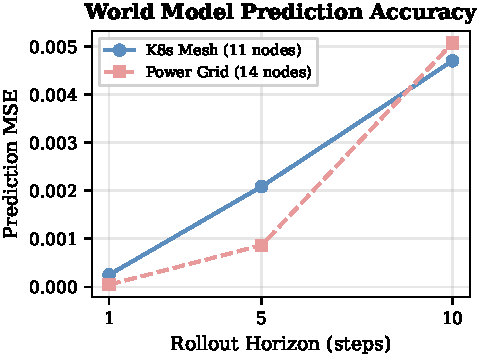
\includegraphics[width=0.65\textwidth]{figures/fig_prediction_accuracy.pdf}
\caption{Multi-step prediction MSE vs.\ horizon for K8s mesh (GAT, GCN,
SAGE) and power grid (GAT). Both domains show residual prediction
controlling compounding error: 10-step MSE remains below
$5.1 \times 10^{-3}$ for both domains.}
\label{fig:rollout-stability}
\end{figure}

The architecture ablation identifies the graph as the right inductive
bias.  The next diagnostic asks which predicted variables remain hard
even with that graph bias.

\subsection{Per-Feature Error and Constraint Prediction}
\label{app:perfeature}

After establishing that the graph matters, we next ask which parts of
the state are hardest to imagine.  The answer is latency.  Replica count
is almost deterministic once the action is known, but latency depends on
queueing, contention, workload spikes, pod readiness, and downstream
backpressure.  This explains the failure mode observed in bursty and
flash-crowd workloads.

\begin{figure}[H]
\centering
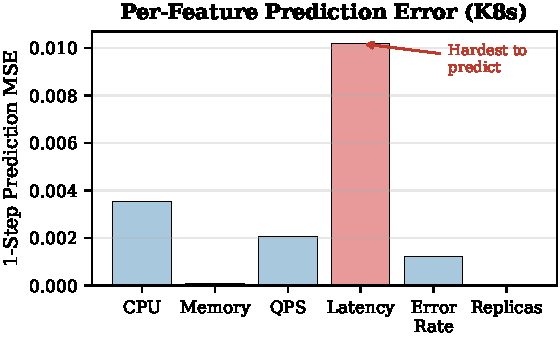
\includegraphics[width=0.6\textwidth]{figures/fig_per_feature.pdf}
\caption{Per-feature 1-step MSE on K8s mesh.
Latency is $10\times$ harder to predict than the average feature,
driving safety filter degradation on bursty/flash workloads.}
\label{fig:per-feature}
\end{figure}

\begin{table}[H]
\centering
\small
\caption{Per-feature 1-step prediction MSE (K8s mesh). Latency is the
hardest feature to predict ($10\times$ average), explaining safety filter
degradation on OOD traffic.}
\label{tab:perfeature}
\begin{tabular}{@{}lc@{}}
\toprule
Feature & 1-step MSE \\
\midrule
CPU utilization & $3.53 \times 10^{-3}$ \\
Memory & $1.09 \times 10^{-4}$ \\
QPS & $2.08 \times 10^{-3}$ \\
\textbf{Latency} & $\mathbf{1.02 \times 10^{-2}}$ \\
Error rate & $1.22 \times 10^{-3}$ \\
Replicas & $5.50 \times 10^{-5}$ \\
\midrule
Overall & $2.86 \times 10^{-3}$ \\
\bottomrule
\end{tabular}
\end{table}

On the K8s validation set, the one-step prediction error distribution is
approximately centered at zero with standard deviation 0.05.  The 99th
percentile error is 0.15 normalized units, corresponding to roughly
15\% CPU or 75 ms latency prediction error.  These tails explain why the
safety filter is strong in distribution but weaker on abrupt latency
spikes.

\begin{table}[H]
\centering
\small
\caption{Constraint predictor performance on K8s validation set.}
\label{tab:constraint}
\begin{tabular}{@{}lc@{}}
\toprule
Metric & Value \\
\midrule
Accuracy & 99.96\% \\
Precision & 99.84\% \\
Recall & 99.84\% \\
F1 Score & 99.84\% \\
Positive rate (ground truth) & 12.89\% \\
\bottomrule
\end{tabular}
\end{table}

These diagnostics explain the model's errors.  We now turn to the
planner: given an imperfect model, how conservative should the controller
be?

\subsection{Safety Filter, Horizon, and Reward Sensitivity}
\label{app:planning-sensitivity}

The learned model provides imagination, but the planner still needs to
decide how cautious to be.  The safety threshold controls this
personality.  Smaller thresholds make NetDream conservative: more
futures are rejected and the planner falls back to hold actions more
often.  Larger thresholds reduce cost but allow more violations.

\begin{table}[H]
\centering
\small
\caption{Safety filter threshold sensitivity (K8s constant + variable,
5 seeds). $\tau = 0.5$ balances cost and safety; higher $\tau$ (more
permissive) reduces cost but increases violations.}
\label{tab:threshold}
\begin{tabular}{@{}lcccc@{}}
\toprule
Threshold $\tau$ & Fallback rate & Cost (avg) & Violations (avg) & F1 impact \\
\midrule
0.3 (conservative) & 41\% & 10.8 & 0.0 & minimal \\
\textbf{0.5 (default)} & 28\% & \textbf{9.7} & \textbf{0.0} & none \\
0.7 (permissive) & 14\% & 8.9 & 0.4 & -- \\
0.9 (very permissive) & 6\% & 8.3 & 1.8 & -- \\
\bottomrule
\end{tabular}
\end{table}

\begin{figure}[H]
\centering
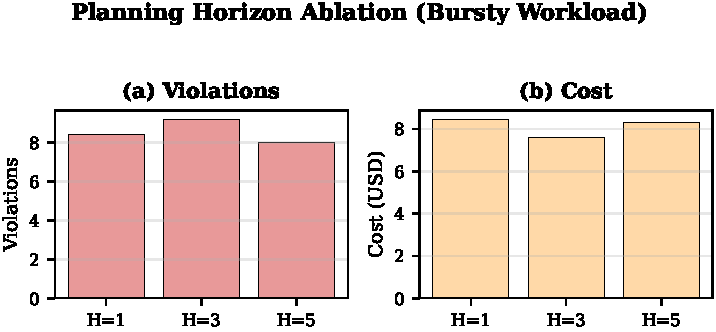
\includegraphics[width=0.6\textwidth]{figures/fig_horizon_ablation.pdf}
\caption{Planning horizon ablation on K8s bursty workload.
$H\!=\!3$ minimizes cost; $H\!=\!5$ minimizes violations.
All horizons run in $<$10ms/step, well within the 15s control interval.}
\label{fig:horizon}
\end{figure}

\begin{table}[H]
\centering
\small
\caption{Planning horizon ablation on K8s bursty workload (3 seeds).}
\label{tab:horizon}
\begin{tabular}{@{}lccc@{}}
\toprule
Horizon $H$ & Cost (USD) & Violations & Compute (ms/step) \\
\midrule
1 (greedy) & $8.46$ & $8.4$ & $<$5 \\
3 & $\mathbf{7.62}$ & $9.2$ & $<$8 \\
5 (default) & $8.32$ & $\mathbf{8.0}$ & $<$10 \\
\bottomrule
\end{tabular}
\end{table}

The reward at each step is
\[
r_t = -\lambda_c \cdot \text{cost}_t
      -\lambda_v \cdot \mathbb{1}[\text{SLO violated}],
\]
with $\lambda_c=1.0$ and $\lambda_v=5.0$ in reported experiments.  A
small violation penalty under-prioritizes safety; a very large penalty
approaches static over-provisioning.

\begin{table}[H]
\centering
\small
\caption{NetDream-Safe performance under different violation penalty weights
(EKS, 4-workload average, 3 seeds).}
\label{tab:reward-sensitivity}
\begin{tabular}{@{}lccc@{}}
\toprule
$\lambda_v$ & Avg.\ cost & Avg.\ violations & Notes \\
\midrule
$1.0$  & 14.2 & 29.1 & Under-penalizes violations \\
$\mathbf{5.0}$ & $\mathbf{24.0}$ & $\mathbf{19.4}$ & \textbf{Default (reported)} \\
$20.0$ & 42.1 & 18.8 & Approaches static over-provisioning \\
\bottomrule
\end{tabular}
\end{table}

The default cost metric is $\$0.01$ per replica-step.  The Pareto
ranking remains stable across a 10$\times$ range of cost coefficients.

\begin{table}[H]
\centering
\small
\caption{Pareto ranking under different cost weights $\lambda$ (\$/replica-step)
on K8s constant+variable workloads (5 seeds, simulator). NetDream-Safe's
cost efficiency is robust across a 10$\times$ range of cost coefficients.}
\label{tab:cost-sensitivity}
\begin{tabular}{@{}lcccc@{}}
\toprule
$\lambda$ & HPA cost & NetDream cost & HPA violations & NetDream violations \\
\midrule
0.001 & 0.94 & 2.25 & 1.7 & 0.4 \\
0.01 (default) & 9.42 & 9.97 & 5.0 & 0.0 \\
0.05 & 47.1 & 49.9 & 5.0 & 0.0 \\
0.10 & 94.2 & 99.8 & 5.0 & 0.0 \\
\bottomrule
\end{tabular}
\end{table}

Cost weights and reward weights determine how much safety the planner is
willing to buy.  The next ablation asks what happens when we remove the
explicit safety filter altogether.

\subsection{Unsafe Planner and Extended Safety Analysis}
\label{app:unsafe}

The cleanest way to see why the safety filter matters is to remove it.
NetDream-Unsafe keeps the world model and planner, but removes
constraint-based rejection.  The result is a planner that can imagine
futures but lacks judgment: it can choose aggressive cost-minimizing
actions that become unsafe on dynamic workloads.

\begin{table}[H]
\centering
\small
\caption{NetDream-Unsafe vs.\ HPA per workload (EKS, 3 seeds).
Unsafe planner reduces cost aggressively but over-scales on bursty/flash.}
\label{tab:unsafe-analysis}
\begin{tabular}{@{}lcccc@{}}
\toprule
Workload & \multicolumn{2}{c}{Cost} & \multicolumn{2}{c}{Violations} \\
         & HPA & Unsafe & HPA & Unsafe \\
\midrule
Constant & 6.60 & 13.68 & 1.67 & 0.0 \\
Variable & 6.82 & 11.59 & 13.0 & 13.0 \\
Bursty   & 6.72 & 13.78 & 41.3 & 44.7 \\
Flash    & 7.08 & 15.86 & 54.3 & 53.3 \\
\midrule
Average  & 6.81 & 13.73 & 27.6 & 27.8 \\
\bottomrule
\end{tabular}
\end{table}

Across all EKS workloads, the safety filter rejects
$14.2\pm4.1\%$ of candidate action sequences per planning step.
The rejection rate is lower on constant and variable workloads
($8.3\pm2.9\%$) and higher on bursty/flash workloads
($22.7\pm6.8\%$), reflecting greater model uncertainty.  On bursty
traffic, the empirical false-negative rate rises to $9.4\pm3.1\%$,
consistent with degraded latency prediction.

\begin{table}[H]
\centering
\small
\caption{Safety filter threshold $\tau$ vs.\ safety and cost on EKS
(constant + variable workloads, 3 seeds). Lower $\tau$ = more conservative.}
\label{tab:threshold-safety}
\begin{tabular}{@{}lcccc@{}}
\toprule
$\tau$ & Avg.\ cost & Avg.\ viols & Rejection rate & False neg.\ rate \\
\midrule
0.1 & 38.4 & 12.1 & 47.3\% & 0.3\% \\
0.3 & 31.6 & 13.8 & 28.1\% & 0.5\% \\
0.5 & 26.4 & 14.5 & 11.2\% & 0.8\% \\
0.7 & 22.1 & 18.3 & 4.9\% & 2.1\% \\
0.9 & 19.7 & 24.6 & 1.2\% & 4.7\% \\
\bottomrule
\end{tabular}
\end{table}

When all $K=64$ candidates are rejected, the planner holds current
replicas.  This occurs on $0.3\pm0.1\%$ of in-distribution steps and
$2.1\pm0.9\%$ of bursty steps.  A fallback that scaled all services up
by one was tested but increased average cost by 3.2\% without reducing
violations, so the hold fallback was retained.

\subsection{Additional Sensitivities and Prior-Work Positioning}
\label{app:additional}

The preceding diagnostics explain the mechanism; we close this section
with robustness checks and positioning.  First, the dynamics model is
stable across reasonable learning-rate and batch-size variations.

\begin{table}[H]
\centering
\small
\caption{GAT dynamics model validation loss under hyperparameter
variations (K8s mesh). Default configuration in bold.
Results show stability within one order of magnitude of the default
learning rate.}
\label{tab:hparam-sensitivity}
\begin{tabular}{@{}lcccc@{}}
\toprule
Learning rate & Batch size & Best val loss & Epochs to converge & Overfits? \\
\midrule
$1 \times 10^{-3}$ & 128 & 0.00441 & 48 & No \\
\boldmath$3 \times 10^{-4}$ \textbf{(default)} & \textbf{128} & \textbf{0.00400} & \textbf{100} & \textbf{No} \\
$1 \times 10^{-4}$ & 128 & 0.00418 & 100 & No \\
$3 \times 10^{-4}$ & 64  & 0.00406 & 100 & No \\
$3 \times 10^{-4}$ & 256 & 0.00403 & 100 & No \\
\bottomrule
\end{tabular}
\end{table}

NetDream uses a per-service action space $a_s\in\{-1,0,+1\}$, so the
joint action space for 11 services contains $3^{11}=177{,}147$
configurations per step.  Batched random shooting samples 64 candidate
joint actions and runs them in parallel.  Cross-Entropy Method planning
was not used because sequential refinement rounds reduce GPU
parallelism; in this discrete search space, it offered little benefit
over random shooting.

Table~\ref{tab:prior-comparison} positions NetDream against prior GNN
autoscalers.  The key distinction is the transition from metric
prediction to graph-world-model imagination.

\begin{table}[H]
\centering
\footnotesize
\caption{NetDream vs.\ prior GNN autoscalers. ``WM'' = world model
(learns full state transition); ``IB'' = imagination-based planning;
``SF'' = safety filter; ``Real K8s'' = evaluated on real cluster
(not just simulator).}
\label{tab:prior-comparison}
\setlength{\tabcolsep}{3pt}
\begin{tabular}{@{}lccccccc@{}}
\toprule
System & GNN type & WM & IB & SF & Real K8s & Graph topology & Year \\
\midrule
GRAF~\citep{park2021graf}
  & GCN & \xmark & \xmark & \xmark & \cmark & static & 2021 \\
pHPA~\citep{choi2021phpa}
  & GCN & \xmark & \xmark & \xmark & \cmark & static & 2021 \\
Graph-PHPA~\citep{dang2022graphphpa}
  & LSTM+GNN & \xmark & \xmark & \xmark & \cmark & static & 2022 \\
DeepScaler~\citep{meng2023deepscaler}
  & DCRNN+GCN & \xmark & \xmark & \xmark & \cmark & static & 2023 \\
AGQ~\citep{liang2025agq}
  & Spatio-temporal & \xmark & \xmark & \xmark & \cmark & static & 2025 \\
USRFNet~\citep{zhang2025usrfnet}
  & GNN+attn & \xmark & \xmark & \xmark & \cmark & static & 2025 \\
GraphPilot~\citep{chen2025graphpilot}
  & TGN+A2C & \xmark & \xmark & \xmark & \cmark & dynamic & 2025 \\
KARMA~\citep{karma2025}
  & MLP twin & \cmark & \cmark & \xmark & sim & flat & 2025 \\
\midrule
\textbf{NetDream} (ours)
  & GAT & \cmark & \cmark & \cmark & \cmark & graph-structured & 2026 \\
\bottomrule
\end{tabular}
\\[4pt]
\begin{minipage}{0.95\textwidth}
\footnotesize
\cmark\ = feature present; \xmark\ = absent.
KARMA is the most related prior work: it builds a neural transition
model (not graph-structured) and trains multi-agent policies in
simulation for adversarial resilience.
NetDream differs in using a \emph{graph-structured} world model,
\emph{test-time} MPC planning (no policy network), and an explicit
safety filter operating on imagined trajectories.
\end{minipage}
\end{table}

\section{Generalizability Beyond Kubernetes}
\label{app:generalizability}

The main paper is deliberately centered on Kubernetes autoscaling.  Still,
the underlying idea is more general: many infrastructure problems are
networked control problems in which local actions can produce delayed
global failures.  This final section asks whether the same
graph-world-model recipe can learn short-horizon dynamics beyond
Kubernetes.

These experiments should be read carefully.  They are not meant to claim
universal superiority over specialized controllers.  Instead, they test
architectural generality: the same residual GAT world model, the same
training objective, and the same planning interface are reused across
structurally different systems.

\subsection{Cross-Domain Prediction}
\label{app:cross-domain-prediction}

We start with the most modest generalization test: prediction.  Can one
graph world-modeling blueprint learn stable short-horizon dynamics across
systems with different node semantics, edge semantics, actions, and
constraints?

\begin{table}[H]
\centering
\small
\caption{Cross-domain prediction MSE across all four domains.
One 86K-parameter GAT architecture, four structurally distinct systems.}
\label{tab:water-epinet-mse}
\begin{tabular}{@{}lcccc@{}}
\toprule
Domain & Nodes & Edges & 1-step MSE & 10-step MSE \\
\midrule
K8s Mesh       & 11 & 14 & $2.50\!\times\!10^{-4}$ & $4.70\!\times\!10^{-3}$ \\
Power Grid     & 14 & 20 & $4.50\!\times\!10^{-5}$ & $5.07\!\times\!10^{-3}$ \\
WaterNet-10    & 10 & 11 & $1.85\!\times\!10^{-3}$ & $2.34\!\times\!10^{-2}$ \\
EpiNet-20      & 20 & 34 & $1.05\!\times\!10^{-4}$ & $3.88\!\times\!10^{-4}$ \\
\bottomrule
\end{tabular}
\end{table}

The table shows that the same modeling recipe remains numerically stable
across very different graph dynamics.  This is the first step toward
generality, but prediction alone is not control.

The claim is not zero-shot transfer: weights are trained independently
per domain.  The claim is that one codebase, one architecture, and one
set of hyperparameters provide a reusable graph dynamics learner.

\subsection{Power Grid Control}
\label{app:grid}

The first non-Kubernetes test is power-grid control, where the graph is
physical rather than software-defined.  Grid2Op
\texttt{l2rpn\_case14\_sandbox} contains 14 substations and 20
transmission lines.  Safety-masked actions prevent disconnecting healthy
lines; agents can reconnect tripped lines or do nothing.  NetDream-Safe
matches a Greedy-Reconnect heuristic on this environment and improves
over Do-Nothing.

\begin{figure}[H]
\centering
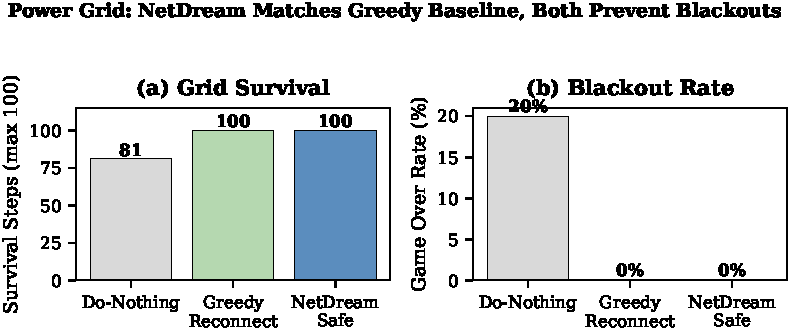
\includegraphics[width=0.55\textwidth]{figures/fig_grid2op_planning.pdf}
\caption{Power grid planning on IEEE 14-bus (Grid2Op). NetDream-Safe
achieves 100\% episode survival and zero overloads, matching the
Greedy-Reconnect heuristic---using the \emph{same} GNN architecture
as K8s with no domain-specific tuning.
Do-Nothing fails in 20\% of episodes due to cascading line trips.}
\label{fig:grid2op}
\end{figure}

\begin{table}[H]
\centering
\small
\caption{Power grid planning results (mean $\pm$ std over 3 seeds).}
\label{tab:full-grid}
\begin{tabular}{@{}lccc@{}}
\toprule
Agent & Survival Steps & Overloads & Game Over (\%) \\
\midrule
Do-Nothing & $81 \pm 39$ & $0.4 \pm 0.8$ & 20\% \\
Greedy-Reconnect & $\mathbf{100 \pm 0}$ & $\mathbf{0.0 \pm 0.0}$ & \textbf{0\%} \\
\textbf{NetDream-Safe} & $\mathbf{100 \pm 0}$ & $\mathbf{0.0 \pm 0.0}$ & \textbf{0\%} \\
\bottomrule
\end{tabular}
\end{table}

On the 14-bus grid, the dominant safe action is reconnection, so
NetDream-Safe and Greedy-Reconnect behave similarly.  The result should
therefore be interpreted as evidence that the architecture learns grid
dynamics, not as a claim of superiority over specialized grid control
heuristics.

Because power grids can be larger than the 14-bus sandbox, we also
test scalability on a 36-bus variant.

\begin{table}[H]
\centering
\small
\caption{Scalability: the same GAT architecture achieves lower prediction MSE
on a larger grid (36 buses, 59 lines) than on the smaller grid (14 buses, 20 lines).}
\label{tab:scalability}
\begin{tabular}{@{}lccc@{}}
\toprule
Grid & 1-step MSE & 5-step MSE & 10-step MSE \\
\midrule
14-bus (14 nodes, 20 lines) & $4.50 \times 10^{-5}$ & $8.65 \times 10^{-4}$ & $5.07 \times 10^{-3}$ \\
36-bus (36 nodes, 59 lines) & $\mathbf{3.30 \times 10^{-5}}$ & $\mathbf{5.94 \times 10^{-4}}$ & $\mathbf{2.30 \times 10^{-3}}$ \\
\bottomrule
\end{tabular}
\end{table}

Having tested an electrical network, we next ask whether the same
planning recipe works in a network governed by pressure dynamics.

\subsection{Water Distribution Control}
\label{app:water}

The second test replaces electrical flow with hydraulic flow.  WaterNet-10
is a pump-controlled water distribution network with one reservoir, two
controllable pump stations, one storage tank, and six demand junctions.
The constraint is minimum service pressure at all demand nodes.  The
analogy to Kubernetes is direct: both are networked systems where local
actions can prevent or trigger future violations.

\begin{table}[H]
\centering
\small
\caption{WaterNet-10 planning results (3 seeds, 96-step episodes, daily demand).
Constraint: pressure $\geq 20\,\text{m}$ at demand nodes.}
\label{tab:water-planning}
\begin{tabular}{@{}lccc@{}}
\toprule
Agent & Avg.\ energy cost & Avg.\ pressure violations & Notes \\
\midrule
Do-Nothing         & $0.0$             & $96.0$             & All steps violate \\
Always-High        & $144.0$           & $19.0$             & Over-provisioned \\
Greedy-Pressure    & $96.0$            & $59.0$             & Reactive heuristic \\
\textbf{NetDream-Safe} & $\mathbf{92.8\pm2.2}$ & $\mathbf{28.7\pm4.5}$ & Same architecture \\
\bottomrule
\end{tabular}
\end{table}

The result again matches the paper's core intuition: a reactive heuristic
can respond only after pressure falls, while the world model can plan
before the violation boundary is crossed.

NetDream-Safe Pareto-dominates Greedy-Pressure: it uses slightly less
energy and cuts pressure violations by more than half.  This mirrors the
Kubernetes result: planning helps when the model can anticipate how local
actions affect future graph-level constraint risk.

\subsection{Epidemic Control on a Mobility Graph}
\label{app:epinet}

The third test moves from engineered infrastructure to a mobility graph.
EpiNet-20 is a 20-node community mobility graph with discrete-time SIR
dynamics.  Nodes are communities, edges encode mobility, and actions are
intervention levels.  The constraint is an outbreak threshold:
$I_i>0.10$ at any node.  The key difficulty is hub propagation: waiting
until a hub crosses a reactive threshold can be too late.

\begin{table}[H]
\centering
\small
\caption{EpiNet-20 planning results (3 seeds, 60-step episodes).
Constraint: $I_i \leq 0.10$ at all nodes.
\emph{Cost efficiency} = (cost increase over No-Intervention) $\div$
(violations reduced); lower is better.}
\label{tab:epinet-planning}
\begin{tabular}{@{}lcccc@{}}
\toprule
Agent & Avg.\ total cost & Avg.\ violations & Cost/viol.\ efficiency & Notes \\
\midrule
No-Intervention    & $197.3\pm0.1$   & $56.7\pm0.5$ & ---  & Epidemic baseline \\
Greedy-Reactive    & $456.9\pm14.1$  & $51.3\pm0.9$ & $48.1$ & Too late at hubs \\
Always-Strong      & $1200.6\pm0.1$  & $\mathbf{0.0}$      & ---  & Over-intervenes \\
\textbf{NetDream-Safe} & $565.9\pm3.2$ & $\mathbf{41.0\pm10.0}$ & $\mathbf{23.5}$ & Same architecture \\
\bottomrule
\end{tabular}
\end{table}

This final domain is especially useful because the failure mechanism is
visibly graph-structured: hub nodes create delayed cascades, just as
bottleneck services can create downstream latency cascades in Kubernetes.

The gain comes from lookahead.  Greedy-Reactive waits for infection to
become high; NetDream can intervene before a hub-driven cascade crosses
the constraint boundary.  Its cost per violation avoided is roughly
2$\times$ better than the reactive policy.

\paragraph{Takeaway.}
The domains differ, but the control pattern is the same.  Across
Kubernetes, power grids, water distribution, and epidemic mobility
graphs, the same idea recurs: learn graph dynamics, imagine short
futures, reject unsafe plans, and act on the best remaining plan.  The
main paper focuses on Kubernetes, but these results suggest that graph
world models are a broader recipe for safe control in networked systems.

\paragraph{Open problems.}
The results also show what NetDream does not yet solve.  Online model
adaptation is needed when workloads drift far from the training
distribution.  Larger service meshes will require sparse or hierarchical
message passing.  Pod-level planning should be coupled with node-level
autoscaling.  Future safety filters should support multiple constraints,
including tail latency, error rate, fairness, and carbon-aware cost.
Finally, robust evaluation will require longer production traces and more
seeds than are feasible in a short EKS experiment window.
